\tikzstyle{MGstyle} =[text centered,draw=blue!50,fill=blue!20,thick,]
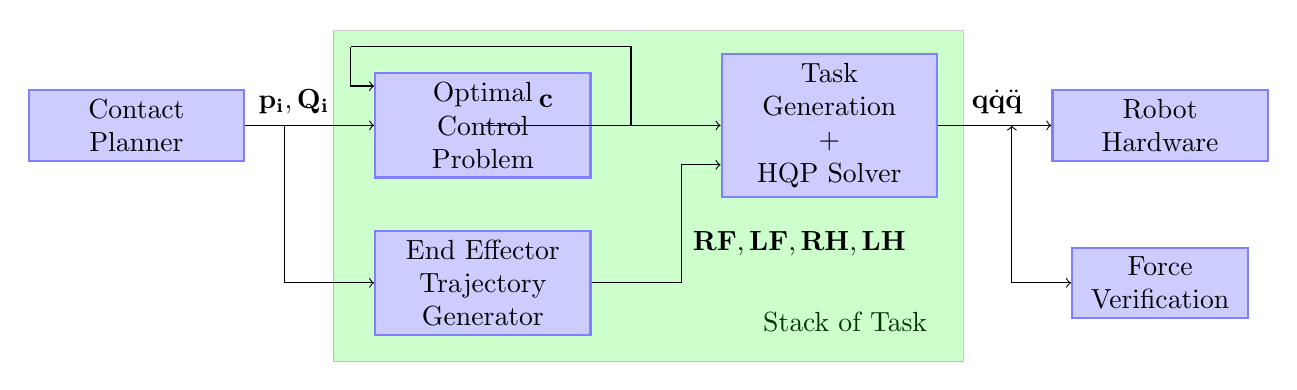
\begin{tikzpicture}[font=\normalsize, node distance=1cm]
% The boxes
  \draw [fill=green,opacity=.2,text opacity=1] (2.5,1.2) rectangle (10.5,-3);
  \node at(9,-2.5) {\textcolor{green!20!black!100}{Stack of Task}};

  \node (cp)   at (0,0) [shape=rectangle,MGstyle,text width=2.5cm]
  {Contact Planner};
  
  \node (eetg)   at (4.4,-2.0) [shape=rectangle,MGstyle,text width=2.5cm]
  {End Effector Trajectory Generator};

  \node (ocp)  at (4.4,0) [MGstyle,text width=2.5cm]
  {Optimal Control Problem};

  \node (gik) at (8.8,0) [MGstyle,text width=2.5cm]
  {Task\\ Generation \\ + \\ HQP Solver};
  
  \node (robot)  at (13.0,0) [MGstyle,text width=2.5cm]
  {Robot Hardware};
  
  \node (fv)  at (13.0,-2.0) [MGstyle,text width=2cm]
  {Force Verification};
  
% The arrows
  % forward
  \draw [->] (cp) -- node [xshift=-0.2cm,yshift=0.3cm] {${\bf p_i},{\bf Q_i}$} (ocp);
  \draw [->] ([xshift=0.5cm]cp.east) |- node {}([xshift=-0.2cm]eetg); 
  \draw [->] (ocp) |- node [xshift=0.8cm,yshift=0.3cm] {${\bf c}$}(gik);
  \draw [- ] (eetg) -| node [xshift=1.5cm,yshift=0.5cm]{${\bf RF},{\bf LF},{\bf RH},{\bf LH}$}([xshift=-0.5cm,yshift=-0.5cm]gik.west);
  \draw [->] ([xshift=-0.5cm,yshift=-0.5cm]gik.west) -- node {}([yshift=-0.5cm]gik.west);
  \draw [->] (gik) -- node [above] {$\begin{matrix}
    {\bf q} \\ \dot{\bf q} \\ \ddot{\bf q}
  \end{matrix}$} (robot);  

  % feedback
  \draw [- ] ([xshift=0.5cm]ocp.east) |- node [above] {} ([xshift=-0.3cm,yshift=1cm]ocp.west);  
  \draw [->] ([xshift=-0.3cm,yshift=1cm]ocp.west) |- node {} ([yshift=0.5cm]ocp.west);
  \draw [->] (fv.west) -| node {} ([xshift=-0.5cm]robot.west);
  \draw [->] ([xshift=-0.5cm]robot.west) |- node {} (fv.west);
\end{tikzpicture}